\documentclass[a4paper,tikz,border=10pt]{standalone}
\usepackage{tikz}
\usetikzlibrary{arrows.meta, positioning, shapes.geometric, calc}

\begin{document}

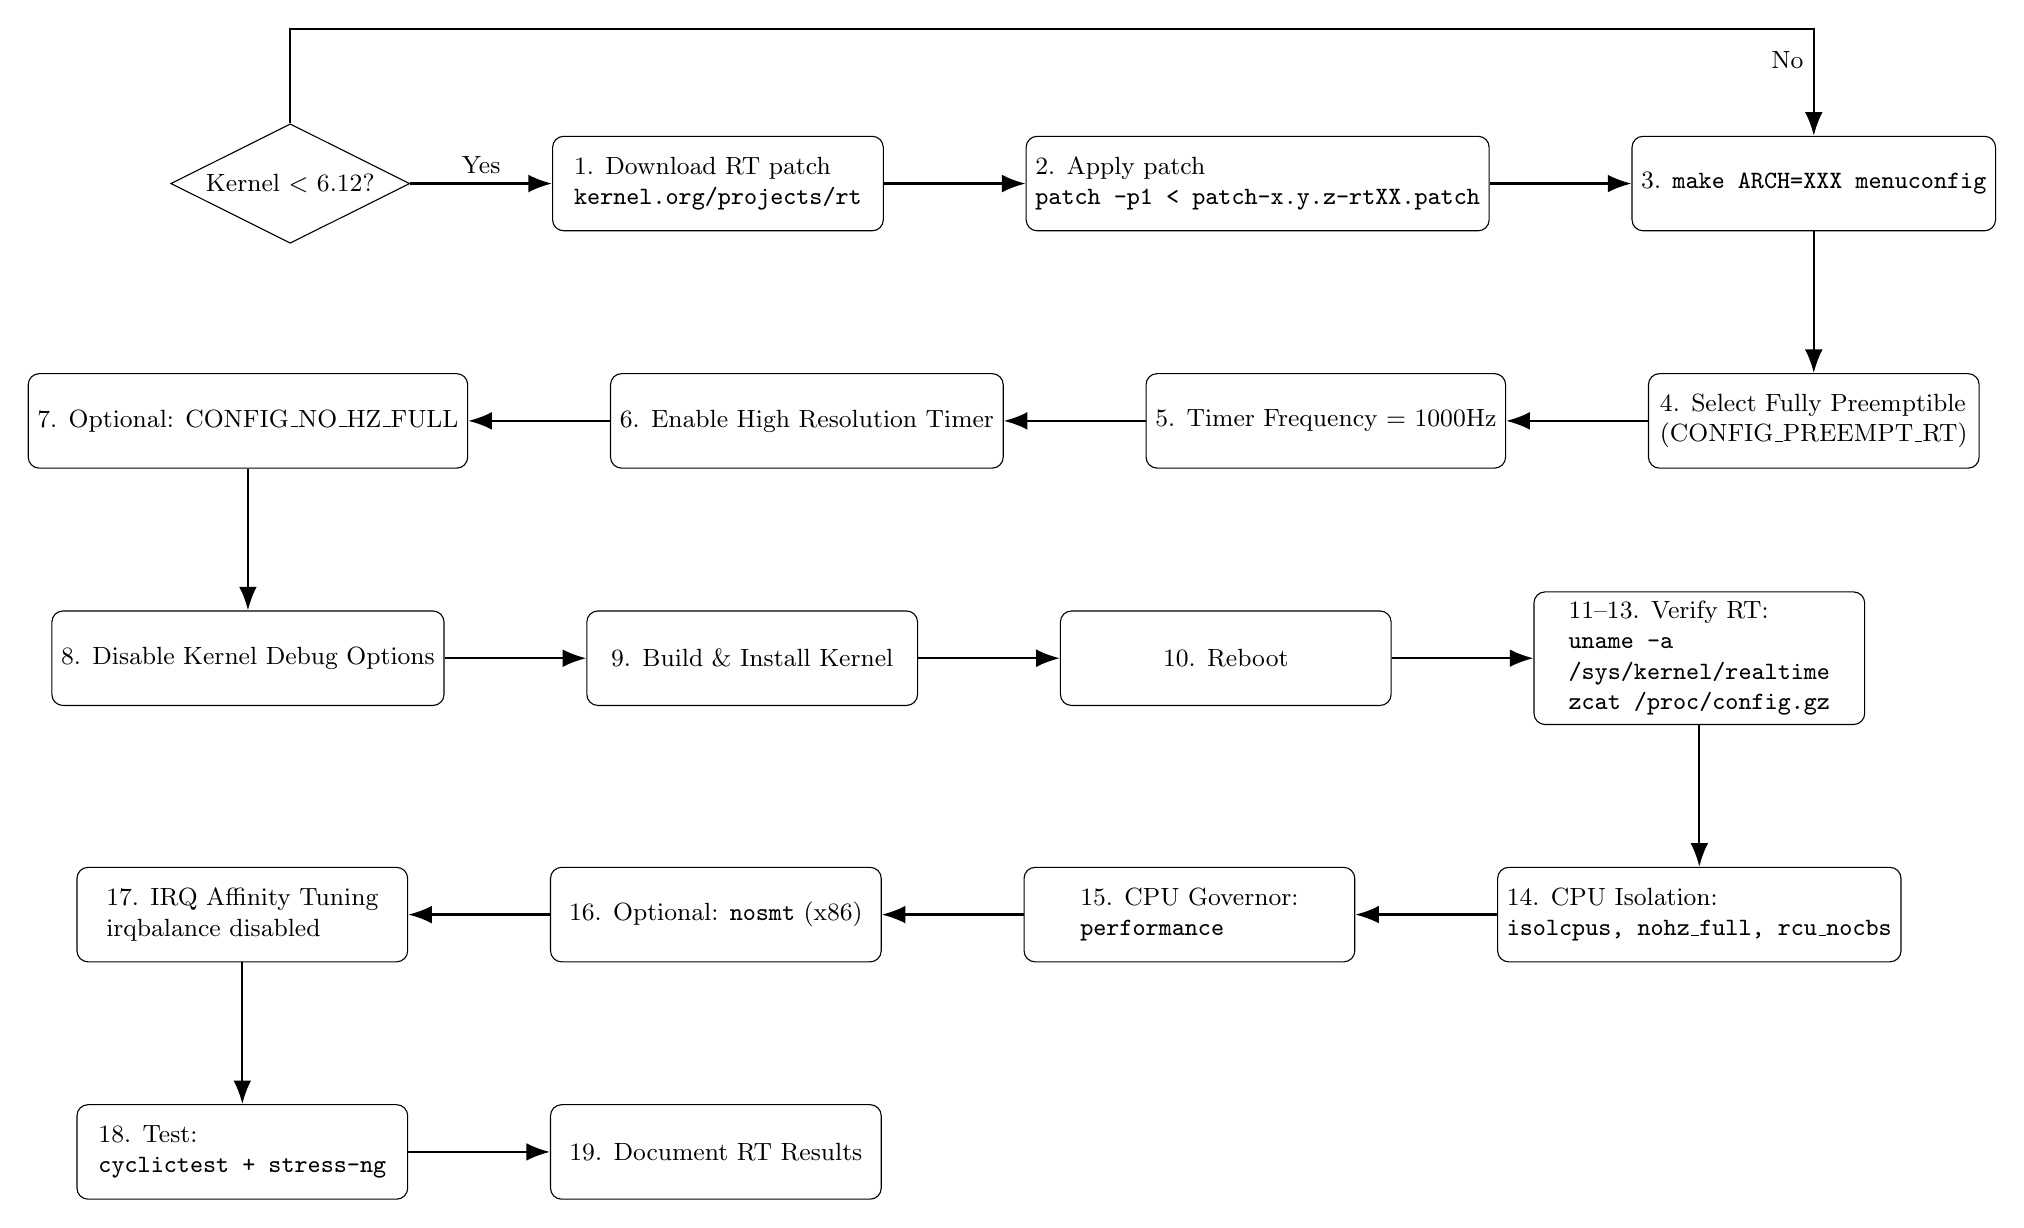
\begin{tikzpicture}[
    node distance=1.8cm and 1.8cm,
    every node/.style={font=\small},
    process/.style={
        rectangle,
        rounded corners,
        draw=black,
        align=left,
        minimum width=4.2cm,
        minimum height=1.2cm
    },
    decision/.style={
        diamond,
        draw=black,
        aspect=2,
        align=center,
        inner sep=2pt
    },
    arrow/.style={
        -{Latex[length=3mm]},
        thick
    }
]

% ---------------- Row 1 (Left to Right) ----------------

\node[decision] (kver) {Kernel $<$ 6.12?};

\node[process, right=of kver] (rtpatch) 
{1. Download RT patch\\
\texttt{kernel.org/projects/rt}};

\node[process, right=of rtpatch] (applypatch) 
{2. Apply patch\\
\texttt{patch -p1 < patch-x.y.z-rtXX.patch}};

\node[process, right=of applypatch] (menuconfig) 
{3. \texttt{make ARCH=XXX menuconfig}};

\draw[arrow] (kver.east) -- node[above]{Yes} (rtpatch);
\draw[arrow] (rtpatch) -- (applypatch);
\draw[arrow] (applypatch) -- (menuconfig);
% \draw[arrow] (kver.north) -| node[left]{No} (menuconfig.north);

\draw[arrow]
    (kver.north)
    -- ++(0,1.2cm)
    -| ($(menuconfig.north)+(0,1.2cm)$)
    -- (menuconfig.north)
    node[pos=0.2,left]{No};


% ---------------- Row 2 (Right to Left) ----------------

\node[process, below=of menuconfig] (preempt)
{4. Select Fully Preemptible\\
(CONFIG\_PREEMPT\_RT)};

\node[process, left=of preempt] (hz)
{5. Timer Frequency = 1000Hz};

\node[process, left=of hz] (hrt)
{6. Enable High Resolution Timer};

\node[process, left=of hrt] (nohz)
{7. Optional: CONFIG\_NO\_HZ\_FULL};

\draw[arrow] (menuconfig) -- (preempt);
\draw[arrow] (preempt) -- (hz);
\draw[arrow] (hz) -- (hrt);
\draw[arrow] (hrt) -- (nohz);

% ---------------- Row 3 (Left to Right) ----------------

\node[process, below=of nohz] (debug)
{8. Disable Kernel Debug Options};

\node[process, right=of debug] (build)
{9. Build \& Install Kernel};

\node[process, right=of build] (reboot)
{10. Reboot};

\node[process, right=of reboot] (verify1)
{11--13. Verify RT:\\
\texttt{uname -a}\\
\texttt{/sys/kernel/realtime}\\
\texttt{zcat /proc/config.gz}
};

\draw[arrow] (nohz) -- (debug);
\draw[arrow] (debug) -- (build);
\draw[arrow] (build) -- (reboot);
\draw[arrow] (reboot) -- (verify1);

% ---------------- Row 4 (Right to Left) ----------------

\node[process, below=of verify1] (bootopt)
{14. CPU Isolation:\\
\texttt{isolcpus, nohz\_full, rcu\_nocbs}};

\node[process, left=of bootopt] (freq)
{15. CPU Governor:\\
\texttt{performance}};

\node[process, left=of freq] (nosmt)
{16. Optional: \texttt{nosmt} (x86)};

\node[process, left=of nosmt] (irq)
{17. IRQ Affinity Tuning \\ irqbalance disabled};

\draw[arrow] (verify1) -- (bootopt);
\draw[arrow] (bootopt) -- (freq);
\draw[arrow] (freq) -- (nosmt);
\draw[arrow] (nosmt) -- (irq);

% ---------------- Row 5 (Left to Right) ----------------

\node[process, below=of irq] (test)
{18. Test:\\
\texttt{cyclictest + stress-ng}};

\node[process, right=of test] (doc)
{19. Document RT Results};

\draw[arrow] (irq) -- (test);
\draw[arrow] (test) -- (doc);

\end{tikzpicture}

\end{document}
